\documentclass{article}
\usepackage{graphicx}
\usepackage{color}
\usepackage{xcolor}

\title{On Foundational Axiomatic Systems for Category Theory}
\author{Christoph Benzm\"uller and Dana Scott}



\begin{document}
\maketitle

\begin{abstract}
Foundational axiomatic systems for category theory are studied. Our novel contributions include
(a) the detection of a previously undiscovered inconsistency in a well known system that has been around for decades, (b) the validation of an alternative system by the second author, and (c) the exploration of novel further alternatives. All of these results were supported by a significant amount of human-computer interaction, in which modern interactive and automated reasoning tools were fruitfully exploited.  
\end{abstract}


\section{Introduction}
The foundational  axiomatic system for category as proposed by Freyd and Scedrov in their 1990 textbook \cite{FreydScedrov90} is either inconsistent or it implies that all morphisms exist. We have detected this novel result by experiments with automated theorem provers. 

An alternative foundational axiomatic systems for category theory has been proposed by the second author already in 1967. In a series of experiments in which automated reasoning tools have been exploited within the proof assistant Isabelle/HOL we have been able to formally validate this system. Moreover, by utilising the available reasoning tools in Isabelle/HOL we have been able to explore and validate interesting further alternatives. These novel alternatives form the core of our contribution.

At the conceptual level this paper exemplifies a new style of explorative mathematics which rests on a significant amount of human-machine interaction with integrated interactive-automated theorem proving technology. Many of the experiments we have conducted were such that the required reasoning was too tedious and time-consuming for humans to carry out with highest precision. It is here were cycles of formalisation and experimentation efforts in Isabelle/HOL provided significant support.

To enable our experiments we have exploited a semantical embedding of free logic in classical higher-order logic, which has recently been proposed \cite{ICMS16}. 

This paper is structured as follows: \ldots

\section{The Issue with the Axiomatic System Freyd and Scedrov}
The following axiomatic system has been proposed by Freyd and Scedrov \cite{ICMS16}:

\begin{figure} \centering
\colorbox{black!20}{
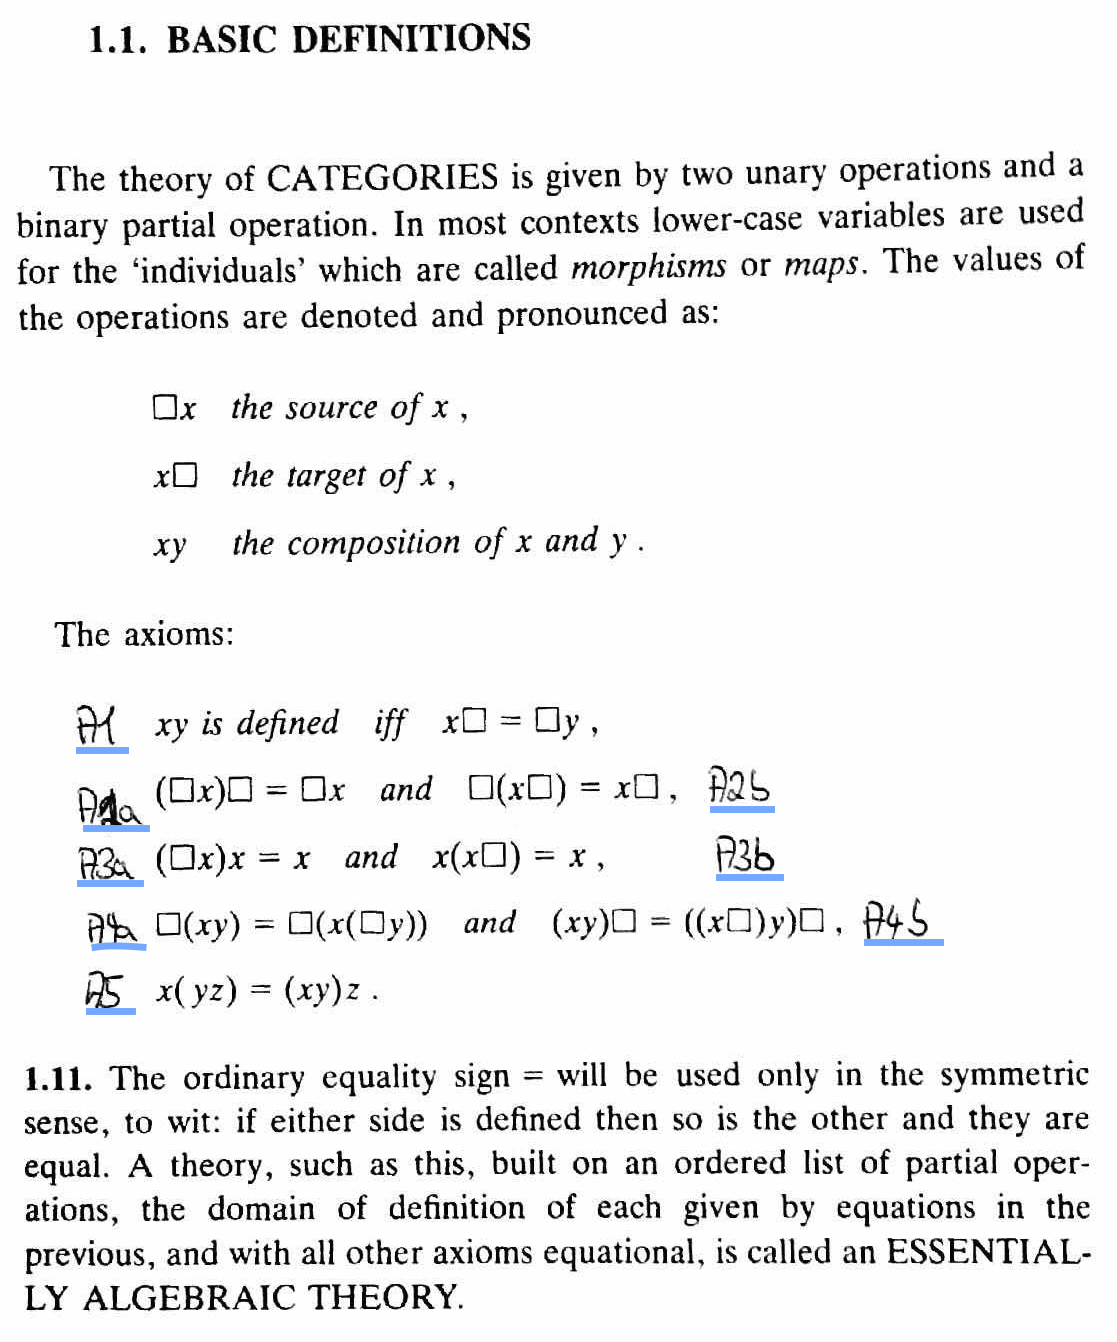
\includegraphics[width=.6\textwidth]{./Images/FreydScedrov2.png}
}
\caption{(Inconsistent) Basic Definitions of Freyd and Scedrov}
\end{figure}


\begin{itemize}
\item First (incorrect) formalisation: \quad \quad \textcolor{red}{$x \approx y$} \quad := \quad
  \textcolor{blue}{$(E(x) \longleftrightarrow E(y)) \wedge x = y$}
\item Freyd/Scedrov want Kleene-Eq: \quad\textcolor{red}{$x \simeq y$} \quad := \quad  \textcolor{blue}{$(E(x) \vee E(y)) \longrightarrow (E(x) \wedge E(y) \wedge x = y)$}
\end{itemize}

\paragraph{1st Series of Experiments}
\textbf{Parameters:} \textcolor{red}{$\approx$}, at least one undefined map ($\star$), definite
description \\
\textbf{Results A:} Redundancies detected \hfill \textcolor{gray}{(in paper)} \\
\textbf{Results B:} Inconsistency detected \hfill \textcolor{gray}{(after paper writing)}

\paragraph{2nd Series of Experiments}
\textbf{Parameters:} \textcolor{red}{$\simeq$}, no $\star$ ($E$ maybe
empty), no definite
description \\
\textbf{Results C:} Consistent if all maps are defined \hfill \textcolor{gray}{(after paper writing)} \\
\textbf{Results D:} Inconsistent if undefined map(s) exist\hfill \textcolor{gray}{(after paper writing)}


\paragraph{3rd Series of Experiments}
\textbf{Parameters:} Scott's own axioms (\textbf{Identity
and Existence in Intuitionistic Logic}, 1977/79), uses 
non-reflexive equality in (A1) and Kleene Equality elsewhere, no $\star$ ($E$ maybe
empty), no definite
description 
\\
\textbf{Results E:} Consistent if all maps are defined \hfill \textcolor{gray}{(after paper writing)} \\
\textbf{Results F:} Still consistent if undefined map(s) exist\hfill \textcolor{gray}{(after paper writing)}




The latter paper also reported on 
earlier experiments on the system by Freyd and Scedrov. However, these experiments were based on a different notion of equality as assumed by Freyd and 


\end{document}